% Appendix A
\chapter{Installation Instructions}
\label{appendix:installation}

This appendix provides instructions for setting up the development environment used in the experiments.

\section{Virtual Machine Setup}

\begin{enumerate}
    \item Download and install \textbf{VirtualBox} from the official website:

    \begin{quote}
        \url{https://www.virtualbox.org/wiki/Downloads}
    \end{quote}

    \item Import the provided virtual machine image (\texttt{dev.ova}) into VirtualBox. A step-by-step guide 
    for importing \texttt{.ova} files can be found here:
    \begin{quote}
        \url{https://chenweixiang.github.io/docs/How_to_Import_and_Export_OVA_Files_in_VirtualBox.pdf}
    \end{quote}
\end{enumerate}

\noindent Once the virtual machine is imported, you can launch the pre-configured development environment to 
reproduce experiments, build the workspace, and run simulations.

%----------------------------------------------------------------------------------------
%	SECTION 2
%----------------------------------------------------------------------------------------
\section{Virtual machine Launch}
Once the virtual machine is imported successfully, go ahead and click the \textbf{Start} button (See Fig:\ref{fig:main_window}). 
\begin{figure}[h]
    \centering
    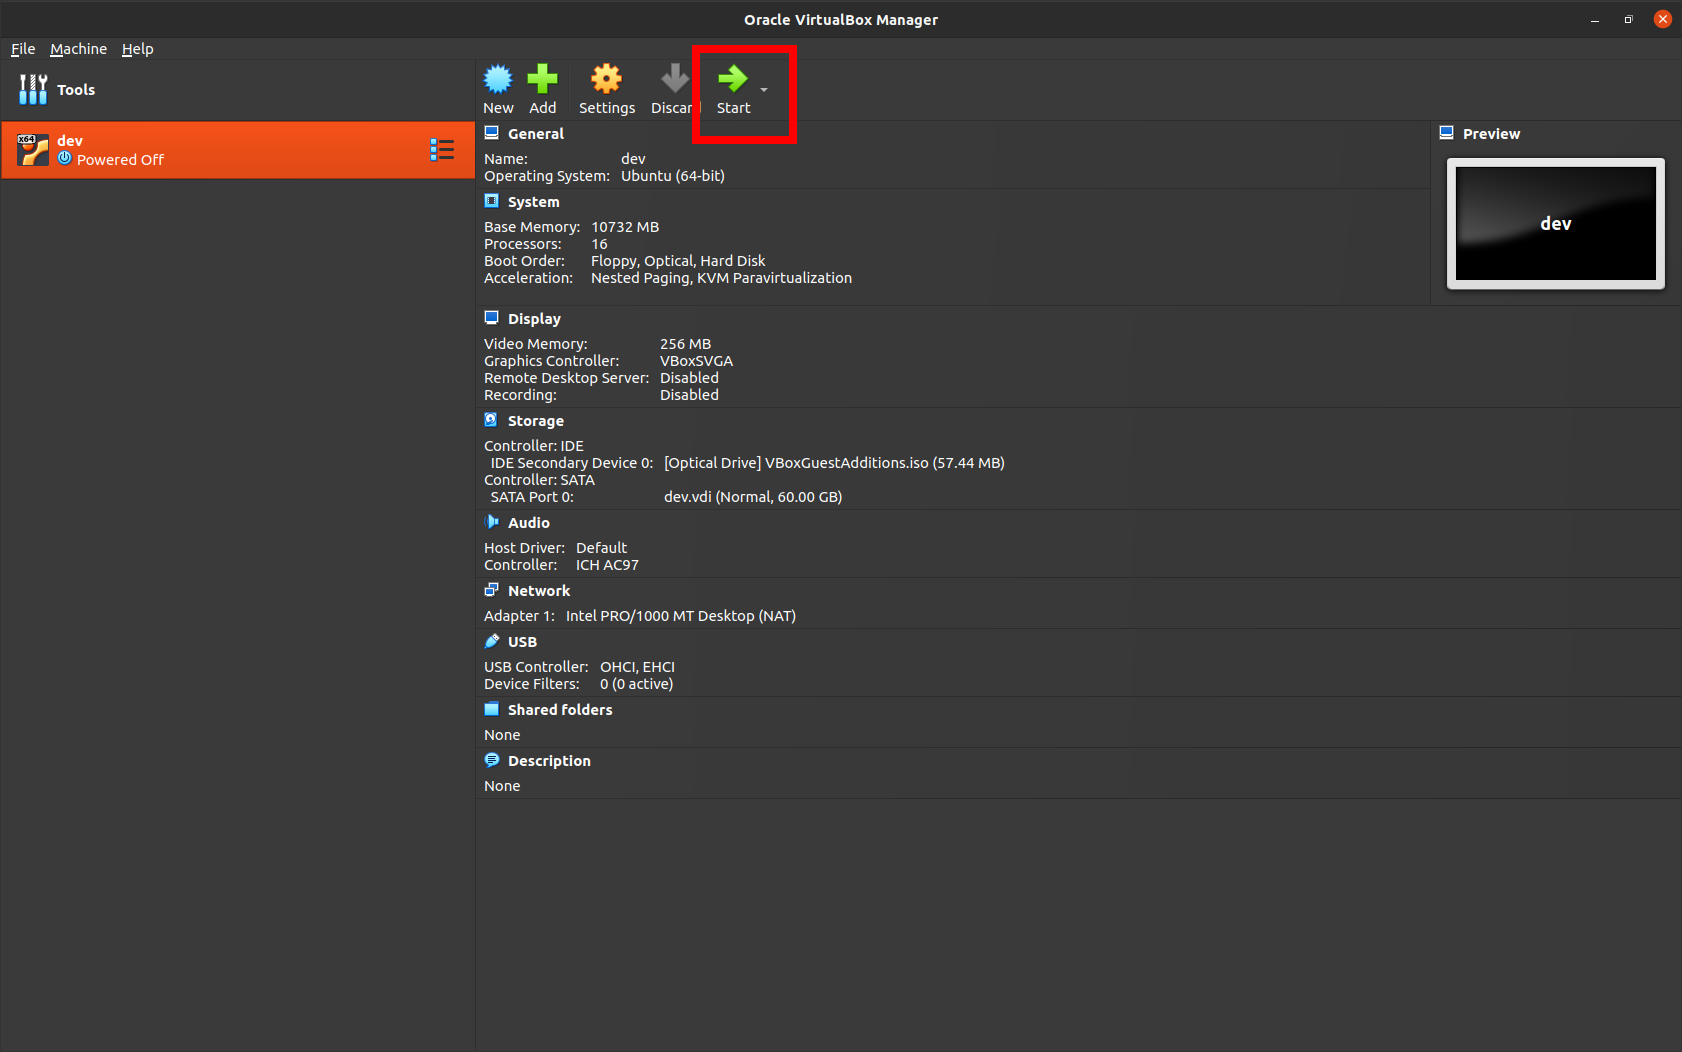
\includegraphics[width=1.0\textwidth]{Figures/vm_launch.png}
    \caption{Virtual Box main window}
    \label{fig:main_window}
\end{figure}
This will launch a new virtual box window where the system is running Ubuntu 20.04. The login the details are as follows:
\begin{itemize}
    \item \textit{User name}: dev
    \item \textit{Password}: thws
\end{itemize}

\noindent Arena-rosnav and Visual Studio Code are fully installed in this virtaul machine and are can be used now.




% Main appendix title
\chapter{Implementation Details of Social Layer Integration in Arena-Rosnav}

\label{AppendixA} % For referencing this appendix elsewhere, use \ref{AppendixA}

\label{appendix:social_layer}

This appendix documents the step-by-step procedure for integrating the social navigation layer into the costmap 
using the Arena-Rosnav simulation framework. The configuration enables socially-aware robot navigation by 
leveraging proxemic behavior modeling.

%----------------------------------------------------------------------------------------
%	SECTION 2
%----------------------------------------------------------------------------------------
\section{Repository Setup}
%-----------------------------------
%	SUBSECTION 1
%-----------------------------------
\subsection*{Step 1: Clone the \texttt{people} repository}

Clone the \href{https://github.com/DLu/people/tree/noetic}{\texttt{people}} repository into the utilities folder:

\begin{lstlisting}[language=bash]
    cd ~/arena_ws/src/arena/utils
    git clone -b noetic https://github.com/DLu/people.git
\end{lstlisting}

This repository provides the \texttt{people\_msgs} message type which must be published on the \texttt{/people} 
topic. For documentation, see: \url{https://docs.ros.org/en/api/people_msgs/html/msg/People.html}.


%-----------------------------------
%	SUBSECTION 2
%-----------------------------------

\subsection*{Step 2: Clone the \texttt{navigation\_layers} repository}

Clone the \href{https://github.com/DLu/navigation_layers/tree/noetic}{\texttt{navigation\_layers}} repository:

\begin{lstlisting}[language=bash]
    cd ~/arena_ws/src/arena/utils/navigation
    git clone -b noetic https://github.com/DLu/navigation_layers.git
\end{lstlisting}

This repository provides the \texttt{social\_navigation\_layers} package, which includes the Proxemic and Passing layers. 
See documentation: \url{http://wiki.ros.org/social_navigation_layers}.


%----------------------------------------------------------------------------------------
%	SECTION 2
%----------------------------------------------------------------------------------------
\section{Publishing \texttt{people\_msgs} from Pedsim}
%-----------------------------------
%	SUBSECTION 
%-----------------------------------
\subsection*{Step 3: Modify the \texttt{pedsim\_simulator}}

Find the simulator:

\begin{lstlisting}[language=bash]
    rospack find pedsim_simulator
\end{lstlisting}

Modify the following files to publish \texttt{people\_msgs}:
\begin{itemize}
  \item \texttt{src/simulator.cpp}
  \item Corresponding header file
\end{itemize}

Ensure the message is published on the \texttt{/people} topic.



%----------------------------------------------------------------------------------------
%	SECTION 2
%----------------------------------------------------------------------------------------
\section{Rebuild Workspace}
%-----------------------------------
%	SUBSECTION 
%-----------------------------------
\subsection*{Step 4: Rebuild with \texttt{catkin build}}

\begin{lstlisting}[language=bash]
    cd ~/arena_ws
    catkin build
\end{lstlisting}











%----------------------------------------------------------------------------------------
%	SECTION 2
%----------------------------------------------------------------------------------------
\section{Costmap Configuration}

\subsection*{Step 5: Add Social Layer Plugins}
%-----------------------------------
%	SUBSECTION 
%-----------------------------------
Edit the costmap parameters file for the robot (e.g., Jackal):

\texttt{/home/dev/arena\_ws/src/arena/simulation-setup/entities/robots \\
/jackal/configs/costmaps/global\_costmap\_params.yaml} \\

Add the following plugin:

\begin{lstlisting}[language=bash]
    - { name: proxemic_layer, type: 
    "social_navigation_layers::ProxemicLayer" }
\end{lstlisting}

Parameters for each layer are configured in: \texttt{costmap\_common\_params.yaml}

\section{Launching and Runtime Adjustment}
%-----------------------------------
%	SUBSECTION 
%-----------------------------------
\subsection*{Step 6: Launch the Simulation}

First, source the workspace and activate the virtual environment if needed:

\begin{lstlisting}[language=bash]
    source ~/arena_ws/devel/setup.bash
    roslaunch arena_bringup start_arena.launch
\end{lstlisting}
%-----------------------------------
%	SUBSECTION
%-----------------------------------
\subsection*{Step 7: Use \texttt{rqt\_reconfigure} for Dynamic Parameters}

Open a new terminal and run:

\begin{lstlisting}[language=bash]
    rosrun rqt_reconfigure rqt_reconfigure
\end{lstlisting}

This allows for real-time adjustment of social navigation parameters.

